\begin{frame}
	\frametitle{Bref historique}
	\only<1>{
		\paraTitle{Sur le boosting}
		\begin{itemize}
			\itemperso{1989}Boosting (R. Schapire)
			\itemperso{1996}AdaBoost (Y. Freund et R. Schapire)
			\itemperso{1999}GBM (L. Breiman puis J. Friedman)
			\itemperso{2014}XGBoost (T. Chen)
		\end{itemize}
	}
	\only<2->{
		\paraTitle{Pour XGBoost}
		\begin{itemize}
	}
		\only<2->{
			\itemperso{Mars 2014}Premières release
			\itemperso{Mai 2014}Python
		}
		\only<3->{
			\itemperso{Septembre 2014}Parallélisation, R
			\itemperso{Mai 2015}YARN, gestion HDFS, SKLearn wrapper
		}
		\only<4->{
			\itemperso{Janvier 2016}API JAVA, amélioration R et Python
			\itemperso{Juillet 2016}C++11, JVM Package (JAVA et Scala)
		}
	\only<2->{
		\end{itemize}\vspace*{\fill}
	}
	\only<2>{
		\rule{0pt}{0pt}\hfill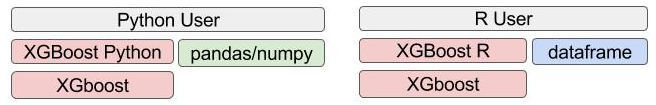
\includegraphics[width=.8\textwidth]{images/implementation/v1}\hfill\rule{0pt}{0pt}
	}
	\only<3>{
		\rule{0pt}{0pt}\hfill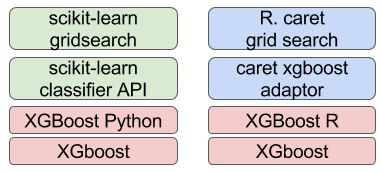
\includegraphics[width=.6\textwidth]{images/implementation/v2}\hfill\rule{0pt}{0pt}
	}
	\only<4>{
		\rule{0pt}{0pt}\hfill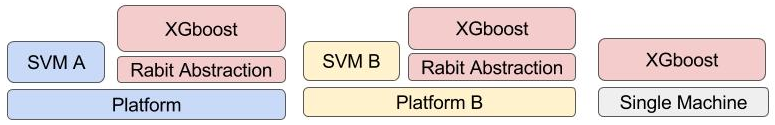
\includegraphics[width=.8\textwidth]{images/implementation/v3}\hfill\rule{0pt}{0pt}
	}
	\only<2->{
		\vspace*{\fill}\rule{0pt}{0pt}

		\rule{0pt}{0pt}\hfill{\fontsize{.15cm}{0cm}\selectfont{\textit{Source : \texttt{http://homes.cs.washington.edu/\~tqchen/2016/03/10/story-and-lessons-behind-the-evolution-of-xgboost.html}}}}
	}
\end{frame}

\begin{frame}
	\frametitle{Des syntaxes proches}
	%bst = xgb.train(param, dtrain, num_round, watchlist)
	%bst <- xgboost(data = train$data, label = train$label, max_depth = 2, eta = 1, nrounds = 2,
    %           nthread = 2, objective = "binary:logistic")
    %bst = xgboost(dtrain, num_round, param = param, watchlist = watchlist,
    %          metrics = ["logloss", "error"])
\end{frame}

\begin{frame}
	\frametitle{Trois familles de paramètres}
	\paraTitle{Paramètres génériques}
	
	Pour définir par exemple quelle méthode Boosting sera utilisée.
	
	\paraTitle{Paramètres liés au Boosting}
	
	Pour paramétrer le booster choisi.
	
	\paraTitle{Paramètres liés à l'apprentissage}
	
	Dépend de la tâche d'apprentissage (classification,...).
\end{frame}

\begin{frame}
	\frametitle{Paramètres génériques}
	\begin{itemize}
		\itemperso{\texttt{Booster}}Linéaire ou arbre.\vspace*{.2cm}
		\itemperso{\texttt{Silent}}Affichage de messages.\vspace*{.2cm}
		\itemperso{\texttt{Nthread}}Par défaut le maximum possible.\vspace*{.2cm}
	\end{itemize}
\end{frame}

\begin{frame}
	\frametitle{Paramètres liés au Boosting}
	\textit{Pour celui sur les arbres. Douze paramètres utiles...}\vspace*{.2cm}

	\begin{itemize}
		\itemperso{\texttt{eta}}Contrôle du niveau d'apprentissage.
		\itemperso{\texttt{Min\_child\_weight}}Pour contrôler l'over/under-fitting
		\itemperso{\texttt{Max\_depth}}Pour contrôler l'over-fitting.
		\itemperso{\texttt{Subsample}}Fraction d'observations à utiliser pour les arbres.
		\itemperso{\texttt{Lambda}}Pour de la régularisation.
		\itemperso{...}
	\end{itemize}
\end{frame}

\begin{frame}
	\frametitle{Paramètres liés à l'apprentissage}
	\begin{itemize}
		\itemperso{\texttt{Objective}}Fonction objectif à minimiser (linéaire, softmax, softprob,...).
		\itemperso{\texttt{Eval\_metric}}Métrique d'évaluation (erreur MSE, MAE, LogLoss, AUC,...).
		\itemperso{\texttt{Seed}}Pour l'aléatoire.
	\end{itemize}
\end{frame}

\begin{frame}
	\frametitle{Quelques bonnes pratique}
	\begin{itemize}
		\itemperso{1.}Fixer un niveau d'apprentissage élevé
		\itemperso{2.}Trouver le nombre optimal d'arbres
		\itemperso{3.}Gérer les paramètres des arbres.
		\itemperso{4.}Gérer les paramètres de régularisation.
		\itemperso{5.}Réduire le niveau d'apprentissage.
	\end{itemize}
\end{frame}